\chapter{Part 3}

\section{Introduction}
%• Very brief introduction of the overall problem setting (< page
%max)

Now describe the setup for the FlexRay modeling part, Figure \ref{fig:FRdia} shows the most important given parts and also the tree view in Inchron along with the FlexRay bus connections.

\begin{figure}[h!]
	\begin{center}
		
			\begin{tabular}{cc}
				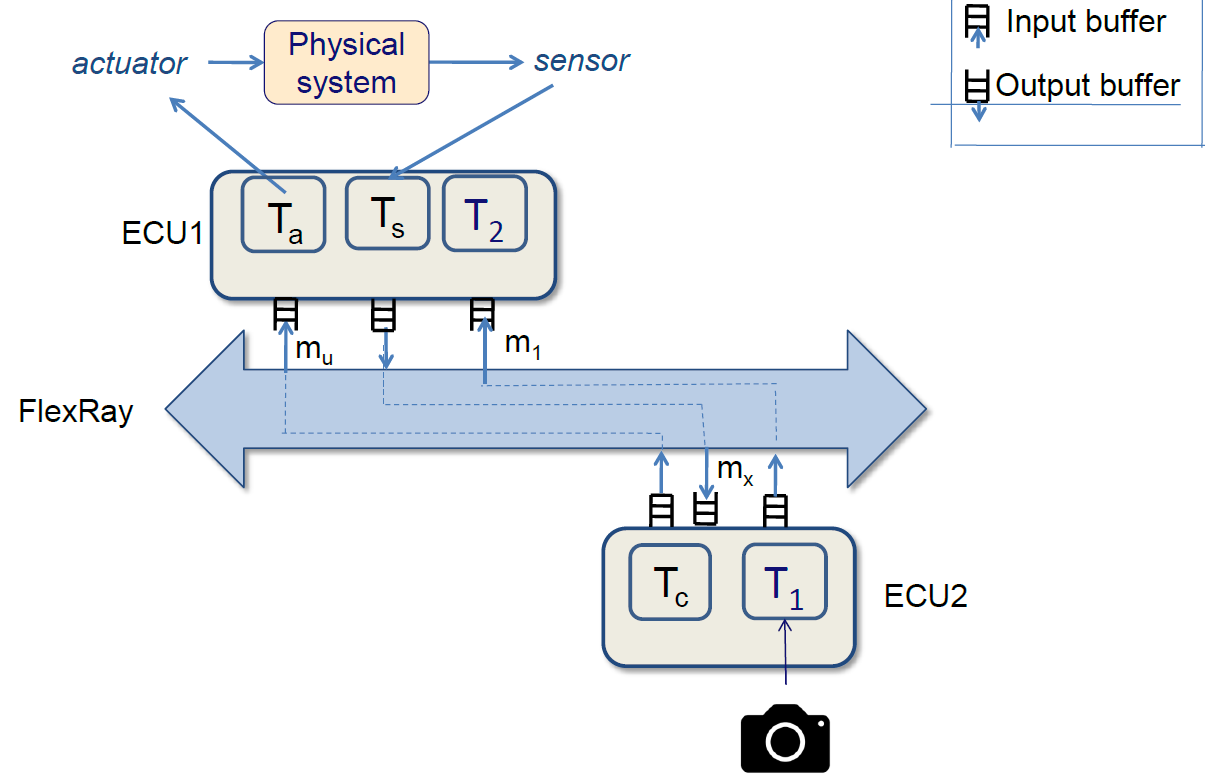
\includegraphics[width=0.5\linewidth]{img/FR-diagram} & 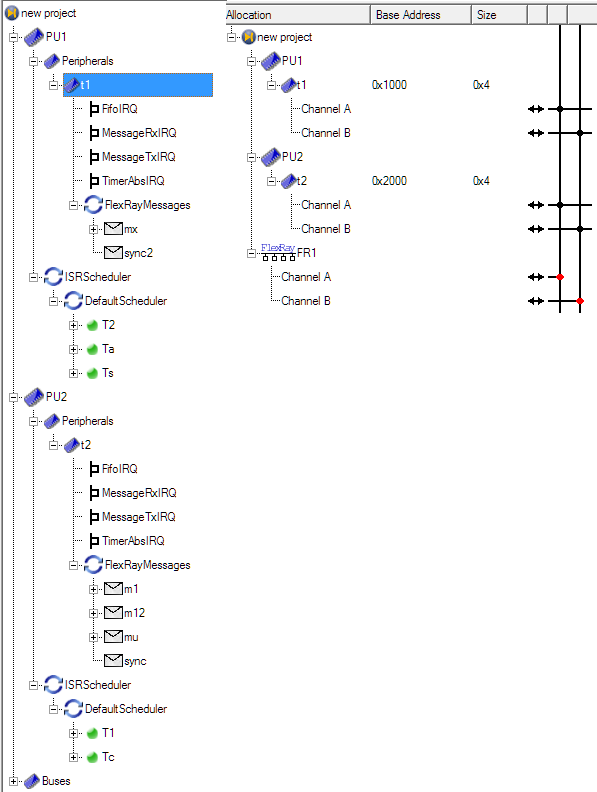
\includegraphics[width=0.35\linewidth]{img/FR-setup}	\\
			\end{tabular}
			\caption{On the left, system diagram and on the right the tree view and architecture of the Inchron project. }
		\label{fig:FRdia}
	\end{center}
\end{figure}


\section{Answer all the questions}


\begin{enumerate}
	\item What is the maximum cycle length possible? 
	
	\item What are the maximum possible durations for:
	
	\begin{enumerate}
			\item static slot?
			
			\item dynamic slot?
			
			\item Network idle time?
	\end{enumerate}	
	
	\item Derive the implicitly defined parameters (e.g., no. of minislots).
	
	\item Why do you need idle phase within a dynamic slot?
	
	\item Does the above parameters conform to FlexRay specification?
	
	\item Answer the above questions in your report Electrical Engineering
\end{enumerate}
What is the maximum cycle length possible? 

What are the maximum possible durations for

static slot?

dynamic slot?

Network idle time?

Derive the implicitly defined parameters (e.g., no. of minislots).

Why do you need idle phase within a dynamic slot?

Does the above parameters conform to FlexRay specification?

Answer the above questions in your report Electrical Engineering



\subsection{Theoretical analysis versus actual implementation}
%Comment on differences from the theoretical analysis and actual implementation


\section{Design decision}
%• Your design decision and justification.

\section{Results}

Firstly: Solution to the design problem. (Include the parameters you have chosen)\\
Secondly: from chronVIEW for your design

\section{Conclusions}